% Author: Izaak Neutelings (October 2021)
% Inspiration
%   "Very special relativity - An illustrated guide", Sander Bais (2007)
%   http://people.uncw.edu/hermanr/GR/Minkowski/Minkowski.pdf
\documentclass[border=10pt,tikz]{standalone}
\usepackage{amsmath} % for \text
\usepackage{etoolbox} % ifthen
\usepackage[outline]{contour} % glow around text
\usetikzlibrary{calc} % for adding up coordinates
\usetikzlibrary{decorations.markings,decorations.pathmorphing}
\usetikzlibrary{angles,quotes} % for pic (angle labels)
\usetikzlibrary{arrows.meta} % for arrow size
\usepackage{xfp} % higher precision (16 digits?)
\contourlength{1.1pt}

\tikzset{>=latex} % for LaTeX arrow head
\colorlet{myred}{red!85!black}
\colorlet{mydarkred}{red!55!black}
\colorlet{mylightred}{red!85!black!12}
\colorlet{myfieldred}{mydarkred!5} % for S' background
\colorlet{myredhighlight}{myred!20} % highlights simultaneity in ladder paradox
\colorlet{myblue}{blue!80!black}
\colorlet{mydarkblue}{blue!50!black}
\colorlet{mylightblue}{blue!50!black!30}
\colorlet{mylightblue2}{myblue!10}
\colorlet{mygreen}{green!80!black}
\colorlet{mypurple}{blue!40!red!80!black}
\colorlet{mydarkgreen}{green!50!black}
\colorlet{mydarkpurple}{blue!40!red!50!black}
\colorlet{myorange}{orange!40!yellow!95!black}
\colorlet{mydarkorange}{orange!40!yellow!85!black}
\colorlet{mybrown}{brown!20!orange!90!black}
\colorlet{mydarkbrown}{brown!20!orange!55!black}
\colorlet{mypurplehighlight}{mydarkpurple!20} 

\begin{document}

% SPACETIME DIAGRAM - EUCLIDEAN ROTATION
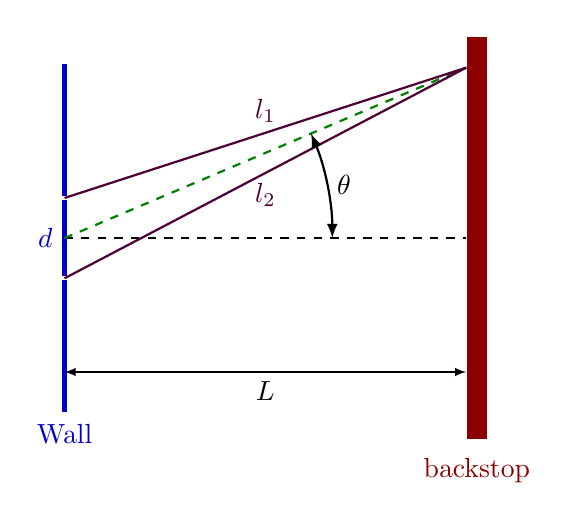
\begin{tikzpicture}[scale=1.7]
    
    \def\sc{0.3};
    \def\L{3};
    \def\x0{0.6};
    \def\th{23};
    \coordinate (X) at ({\L}, {\L*tan(\th)});
    \draw[line width=2, myblue] (0, {-0.95*\sc}) -- (0, {0.95*\sc}) node [midway, left] {$d$};
    \draw[line width=2, myblue] (0, 1.3) -- (0, {1.05*\sc});
    \draw[line width=2, myblue] (0, -1.3) node [below] {Wall}-- (0, {-1.05*\sc}) ;
    \draw[line width=7, mydarkred] (\L+0.08, 1.5) -- (\L+0.08, -1.5) node [below] {backstop};
    \draw[dashed, thick] (0, 0) -- (\L, 0);
    \draw[thick, dashed, mydarkgreen] (0, 0) -- (X);
    \draw[thick, mydarkpurple] (0, \sc) -- (X) node [midway, above] {$l_1$};
    \draw[thick, mydarkpurple] (0, -\sc) -- (X) node[midway, below] {$l_2$};
    \draw[thick, <->] (2, 0) arc (0:{\th}: 2) node [midway, right] {$\theta$};
    \draw[<->] (0, -1) -- ({\L}, -1) node [midway, below] {$L$};



\end{tikzpicture}


\end{document}